%%%%%%%%%%%%%%%%%%%%%%%%%%%%%%%%%%%%%%%%%%%%%%%%%%%%%%%%%%%%%%%%%%%%%%
% How to use writeLaTeX: 
%
% You edit the source code here on the left, and the preview on the
% right shows you the result within a few seconds.
%
% Bookmark this page and share the URL with your co-authors. They can
% edit at the same time!
%
% You can upload figures, bibliographies, custom classes and
% styles using the files menu.
%
%%%%%%%%%%%%%%%%%%%%%%%%%%%%%%%%%%%%%%%%%%%%%%%%%%%%%%%%%%%%%%%%%%%%%%

\documentclass[12pt]{article}

\usepackage{sbc-template}

\usepackage{graphicx,url}

%\usepackage[brazil]{babel}   
\usepackage[utf8]{inputenc}  
\usepackage[normalem]{ulem}
\usepackage{graphicx}
\usepackage{float}
\usepackage[normalem]{ulem}
\useunder{\uline}{\ul}{}

\usepackage[square,sort,comma,numbers]{natbib}

\usepackage[portuguese]{babel}

%#### CONFIGURAÇÃO DE IDIOMA E ACENTUAÇÃO ###

\usepackage[utf8x]{inputenc}
\usepackage[portuguese]{babel}
\usepackage[T1]{fontenc}
\usepackage{indentfirst}

%#### CONFIGURAÇÃO DE GRÁFICOS ###

\usepackage{graphicx}
\usepackage{float} %mais controle sobre posicionamento de imagens
\usepackage{tikz} %para fazer desenhos
\usepackage{bchart} %para graficos em barra horizontal


\usepackage{pgfplots} %pacote grafico poderoso
\pgfplotsset{width=10cm,compat=1.9} %pacote grafico poderoso
\usepgfplotslibrary{external} %Compatibilidade grafica

%#### CONFIGURAÇÕES MATEMÁTICAS ####

\usepackage{amsmath} 
\usepackage{amsfonts} 
\usepackage{amssymb} 

%#### CONFIGURAÇÕES REFERENCIAS BIBLIOGRÁFICAS ####

\usepackage{natbib}

%#### CONFIGURAÇÕES EXTRAS GERAIS ####

\usepackage{multicol} %Usar colunas
\usepackage{color} %%Usar cores
\usepackage{lipsum}
\usepackage{hyperref}
\usepackage{url}
\usepackage{csquotes}
\usepackage{array,multirow} %para gerar tabelas com colunas e/ou linhas mescladas e texto escrito na vertical
%\usepackage{draftwatermark} %Para usar marca d'agua \usepackage[firstpage]{draftwatermark} se quiser apenas na primeira pagina
\usepackage{scalefnt}


\sloppy

\title{Redes de Coautoria da Base SciELO: Avaliação da Colaboração Científica}

\author{Vitor Luiz Pereira Ribeiro}
  
\address{Instituto de Computação -- Universidade Federal de Alagoas
  (IC/UFAL)
  \email{vitor.ribeiro@laccan.ufal.br}
}

\begin{document} 

\maketitle

%\begin{abstract}
  
%\end{abstract}
     
%\begin{resumo} 
  
%\end{resumo}


\section{Introdução}

\subsection{\textbf{Definição do Problema}}~\label{sec:def_Problema}

A colaboração científica é um fenômeno social que tem  por objeto a produção de conhecimento e os cientistas como os principais atores. As redes de coautoria é uma das formas de mensuração e indicação da interação entre esses atores, pelo esforço colaborativo entre pessoas, instituições e países para a geração e publicação de um trabalho científico.

Nos últimos anos vários estudos tem sido realizado para a compreensão deste fenômeno \citep{Maia2008}, buscando entender como ocorre. 
Avançar nos estudos e no entendimento da colaboração científica no Brasil é fundamental para que tenhamos uma ideia mais clara de como este fenômeno vem acontecendo na comunidade científica brasileira, possibilitando a definição e o direcionamento de políticas científicas mais adequadas \cite{Vanz2010}.

O Conselho Nacional de Desenvolvimento Científico e Tecnológico -- CNPq\footnote{http//www.cnpq.br} é o mantenedor da base de Currículos Lattes\footnote{http://lattes.cnpq.br}, a principal fonte de registro dos trabalhos e publicação científica do país. 
Entretanto, a plataforma Lattes não vem apresentando avanços significativos, principalmente pela não disponibilização de dados abertos, assim, impossibilitando a realização de pesquisas que possam descrever o comportamento bibliométrico da ciência no país.
Uma evidência da desatualização do Lattes é a própria plataforma Painel Lattes\footnote{http://estatico.cnpq.br/painelLattes/} que não possui dados atualizados.

A Scientific Electronic Library Online -- SciELO\footnote{http://www.scielo.br} é uma biblioteca eletrônica criada em 1998.
Ela realiza a indexação de um conjunto de periódicos visando o desenvolvimento de uma metodologia comum para a preparação, armazenamento, disseminação e avaliação de literatura científica em formato eletrônico.

No entanto, apesar dos esforços da SciELO em disponibilizar uma ferramenta para o maior conhecimento de métricas biliométricas e a observação do comportamento da colaboração científica, sua plataforma SciELO Analytics\footnote{http://analytics.scielo.br} ainda carece de funcionalidades para a visualização de redes de coautoria, considerando o aspecto interinstituicional.

Diante do contexto supra explanado, essa pesquisa visa a proposta de um modelo da avaliação da colaboração científica com base na análise de redes de couatorias interinstituições do Brasil. 
Buscamos responder precipualmente as seguintes questões:
\begin{itemize}
\item Como se caracterizam as redes de coautoria na base SciELO?
\item Quais as propriedades e métricas que indicam a evolução das redes de coautoria ao longo do tempo?
\item Como se observa as comunidades de colaboração científica a partir das redes de coautoria?
\end{itemize}

\subsection{\textbf{Revisão da Literatura}}~\label{revisao}

A bibliometria é uma campo de conhecimento multidisciplinar com origem na biblioteconomia e na ciência da informação, que aplica métodos estatísticos e matemáticos para analisar e construir indicadores sobre a dinâmica e evolução da informação científica e tecnológica de determinadas disciplinas, áreas, organizações ou países.

\cite{pritchard1969statistical} descrevem que bibliometria é o tratamento quantitativo das propriedades da escríta científica publicada e do comportamento que lhe é inerente. 
%%% ACF A frase que segue não faz sentido
\cite{osareh1996bibliometrics} define a biliometria como o estudo dos padrões das publicações científicas aplicando análises quantitativas e estatísticas. %Lancaster (1977: 353)% 
%%% VLR frase rescrita 

Estudos e análises bibliométricas podem ser empregadas a diversas áreas do conhecimentos com abordagens como avaliação da produtividade científica, análise de citações e cocitações, redes de coautoria, análise de fatores de impacto, dentre outros. A bibliometria possui estreitas relações com as áreas de cienciometria (ou cientometria), infometria, webometria, patentometria, e altmetria.

Em redes de coautoria \textit{(co-authorship network)}, conforme \cite{Barabasi2001}, estudos vêm apresentando evoluções significativas, entretanto de maneira muito fragmentada, se concentrando em uma característica da rede por vez. 
O autor ressalta também a complexidade envolvida em virtude da velocidade de crescimento das redes, comparando-as como o comportamento da rede \textit{World Wide Web}, visto que há de se considerar os vários formatos das bases de dados e suas indexações.
Fica, assim, configurado o desafio para estudos relacionados a este tema.



\subsection{\textbf{Contribuições}}~\label{contribuicao}
  
Neste trabalho propomos desenvolver um estudo para avaliação da colaboração científica por meio de redes de coautoria, com as seguintes caraterísticas:

\begin{itemize}
\item Reprodutibilidade com a definição da instituição vértice de referência.
\item Definição do intervalo temporal em anos para análises comparativas.
\item Explanar as características e métricas quantitativas das redes pelo aspecto da colaboração científica.
\end{itemize}

\subsection{\textbf{Objetivos}}~\label{obetivos}

O objetivo desta pesquisa é a proposta da criação de um estudo modelo avaliativo do comportamento das redes de coautoria na base de dados objeto desse estudo, considerando alguns objetivos secundários, são eles:

\begin{itemize}
\item Avaliação das propriedades e indicadores de redes de coautoria inter instituição.
\item Visualização por comunidades definidas pelas regiões geográficas do Brasil.
\item Caracterização da colaboração a partir dos resultados de métricas bibliométricas de redes de coautoria.
\end{itemize}

\section{Fundamentação Teórica}

A fundamentação deste trabalho encontra-se respaldado na teoria dos grafos e na análise de redes sociais. 


\subsection{Teoria dos Grafos}

O estudo de redes complexas é um tema  que abrange diversas áreas de conhecimento, tais como a ciência da computação, matemática, física, biologia e sociologia. 
O termo ``redes complexas'' refere-se a um grafo que apresenta uma estrutura topográfica não trivial, composto por um conjunto de vértices (nós) que são interligados por meio de arestas \cite{barabasi2003everything}. 
O estudo de redes na forma de grafos é um dos pilares da matemática discreta e teve início em 1735, quando Euler propôs uma solução para o problema das pontes de Königsberg, originando a teoria dos grafos.

Em teoria de grafos, temos que um grafo é o conjunto de G(V,E) onde G = Grafos, V = Vértices e E = Edge (ou arestas / ligações), onde V é um conjunto não vazio de objetos denominados vértices (ou nós) e E é um subconjunto de pares não ordenados de V. Neste entendimento temos que grafos pode serem caracterizados no prisma de algumas propriedades como por exemplo o comportamento da ligação das arestas como direcional ou não direcional.

Redes de coautoria se caracteriza por ligação não direcional, ou seja, que independe de quem seja o ponto de origem para o destino da ligação, pois devemos para a proposta deste trabalho, considerar que se uma instituição publicou um artigo em coautoria com outra instituição, a recíproca é verdadeira e não há distinção de qual tem propriedades valoradas, como a iniciativa ou mesmo o grau de participação do coautor na publicação em tela.


As figuras abaixo representam a plotagem de grafos apresentando a visão da abordagem de coautorias intra-regional conforme a Figura \ref{grafo1}, e coautorias inter-regional vide Figura \ref{grafo2}, onde S é a representação da região da instituição, X os autores (vértices ou nós) e as arestas/ligações representam a relação de coautoria entre eles.


\begin{figure}[H]
\centering
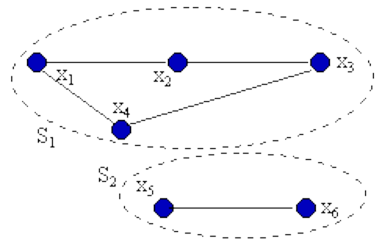
\includegraphics[scale=0.6]{images/intra-grafo.gif}
\caption{Grafo com representação de Rede de Coautoria intra regional}
\label{grafo1}
\end{figure}

\begin{figure}[H]
\centering
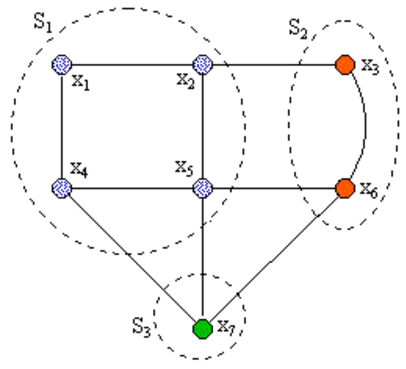
\includegraphics[scale=0.6]{images/inter-grafo.gif}
\caption{Grafo com representação de Rede de Coautoria inter regional}
\label{grafo2}
\end{figure}

\subsection{Análise de Redes Sociais}

Conforme \cite{Silva2006}, a análise de redes sociais interessa a pesquisadores de vários campos do conhecimento que, na tentativa de compreender o seu impacto sobre a vida social, deram origem a diversas metodologias de análise que têm como base as relações entre os indivíduos, em uma estrutura em forma de redes.

A análise de redes sociais (ARS ou SNA, da expressão em inglês \textit{Social Network Analysis)} é uma abordagem oriunda da sociologia, da psicologia social e da antropologia. \cite{freeman1996some,wasserman1994social}. ARS não é algo recente, há estudos, como o trabalho de \cite{otte2002social} que buscou desde a década de 1970, análises de redes de informação, de pesquisadores e de citações, como também de redes de coautoria.

 Redes de couatoria utiliza-se da análise de redes sociais embasada nas propriedades e aplicações de redes complexas, a qual vemos a seguir.


\begin{figure}[H]
\centering
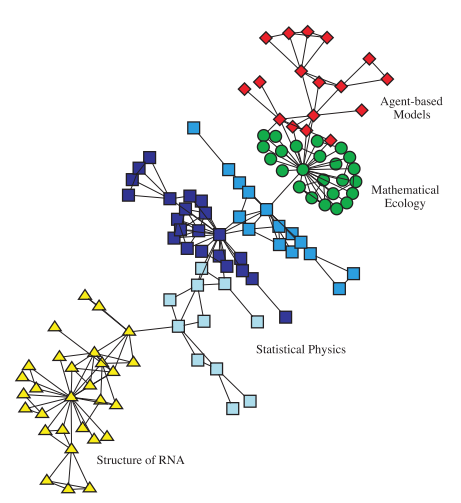
\includegraphics[scale=0.6]{images/rede-newman.PNG}
\caption{Pequena Rede de Coautoria de Newman}
\label{rede1}
\end{figure}


\subsection{Redes Complexas}

No contexto da teoria de redes complexas, uma rede corresponde a um grafo, que se representa por um conjunto de nós ligados por arestas, que em conjunto formam uma rede.  Esta rede ou grafo, permite representar relações com fundamento das propriedades dos vários tipos de grafos e como são constituídos, ou seja, como se agrupam os seus nós e são ligadas suas arestas %\cite{mendes2005fisica}.

%As propriedades de redes complexas às quais utilizaremos nesse trabalho são:
%a)~grau de um nó - é o número de ligações de um nó;
%b)~distribuição da conectividade - forma como se distribuem as ligações pelos nós;
%c)~conectividade média - é dada pela média do número de ligações entre os nós;
%d)~caminho mais curto - é a menor distância entre dois nós de uma rede, dado que poderá haver mais do que um caminho a ligá-los;
%e)~diâmetro - é o comprimento da maior distância entre 2 nós, medidos em número de ligações;
%f)~coeficiente de agregação ou aglomeração \textit{(clustering coefficient)} - é o número de ligações entre os vizinhos mais próximos de um nó;
%g)~redes estáticas/dinâmicas - a rede é estática quando não há variação do número de nós e, é dinâmica, quando é possível modelar o seu crescimento pela análise da variação da sua estrutura ao longo do tempo.

%%% VLR definir se usar o itemize, enumerate ou não usar.

\begin{itemize}
\item Grau de um nó - é o número de ligações de um nó;
\item Distribuição da conectividade - forma como se distribuem as ligações pelos nós;
\item Conectividade média - é dada pela média do número de ligações entre os nós;
\item Caminho mais curto - é a menor distância entre dois nós de uma rede, dado que poderá haver mais do que um caminho a ligá-los;
\item Diâmetro - é o comprimento da maior distância entre 2 nós, medidos em número de ligações;
\item Coeficiente de agregação ou aglomeração \textit{(clustering coefficient)} - é o número de ligações entre os vizinhos mais próximos de um nó;
\item Redes estáticas/dinâmicas - a rede é estática quando não há variação do número de nós e, é dinâmica, quando é possível modelar o seu crescimento pela análise da variação da sua estrutura ao longo do tempo.
\end{itemize}

\section{Colaboração Científica}

Colaboração científica pode ser definida como interação que ocorre dentro de um contexto social entre dois ou mais cientistas, que facilita a partilha de significado e conclusão de tarefas em relação a um objetivo mútuo, compartilhado e organizado. Os cientistas que colaboram também podem trazer metas individuais adicionais para uma colaboração. \cite{Sonnenwald}

Ainda, segundo a autora, a colaboração ocorre dentro do contexto social da ciência, que inclui elementos como a revisão por pares, sistemas de prêmios, paradigmas científicos, políticas de ciência nacionais e internacionais, bem como normas implícitas ao campo disciplinar das instituições de pesquisa e/ou universidades. 

Conforme \cite{Newman2004}, há algum tempo se percebe que a coautoria de artigos em periódicos acadêmicos fornece uma janela sobre padrões de colaboração dentro da comunidade acadêmica. 

Para \cite{Sonnenwald}, estudos da colaboração científica está aumentando, por possuir o potencial de auxiliar a resolução de problemas científicos complexos e promover agendas políticas, econômicas e sociais. 

\section{Metodologia} 

A metodologia utilizada para a presente pesquisa utiliza um modelo exploratório que consiste em quatro etapas cíclicas: 
a)~definição da rede, 
b)~tratamentos de dados da rede; 
c)~determinação das características estruturais e 
d)~inspeção visual \cite{de2018exploratory}.

A definição da rede resultou da coleta dos dados realizada no portal da SciELO\footnote{http://static.scielo.org}. 
Foram  realizados tratamentos desses dados normalizando a padronização os campos da Unidade Federativa (UF). 
A base foi complementada pela informação da localidade geográfica associando os estados (UF) às regiões do Brasil. 
%%% ACF Escreva sempre da forma mais simples e direta possível, a seguinte frase poderia ser "Documentos de origem estrangeira foram definidos como ``Exterior''.
%% Documentos de origem estrangeira foram definidos como ``Exterior''.
%%% VLR Frase reescrita 
%%% VLR documentos do Exterior foram excluídos do escopo

Os dados foram coletados no sítio eletrônico da SciELO a partir do endereço \url{http://static.scielo.org/tabs/tabs_bra}. Os dados associam os documentos publicados em coautoria de um autor com sua respectiva instituição de origem por um ID. O conjunto de dados amostral utilizado para esta pesquisa compreende o período entre 2008 à 2017 e os documentos relacionados as Universidades Federais do país.  

Foi utilizada a linguagem de programação \texttt R, possibilitando que o resultado deste trabalho seja coberto ponta a ponta com a mesmo código, facilitando assim a reprodutibilidade desta pesquisa.

O total de documentos indexados no dados coletados resultou um montante de 1.302.659 documentos indexados, para fins desta pesquisa a amostra determinada resultou um total de xxx documentos.

A produção dos resultados teve por fundamento a teoria dos grafos e na análise de redes sociais, onde buscou a aplicação das métricas de redes complexas, para a compreensão do comportamento das redes de coautoria do presente estudo.

Este trabalho utilizou-se da linguagem \texttt R com o uso dos pacotes \texttt{tidyverse}, \texttt{igraph} e \texttt{ggraph}. A seguir descrevemos as etapas cíclicas proposta por \cite{de2018exploratory} para estudos relacionados ARS.

\subsection{Definição da rede}

As redes objeto de estudo desta pesquisa é a relação de coautoria existentes nos documentos indexados na base de dados da SciELO, objetivando a criação de um modelo exploratório. Foram definidas as redes de coautoria segregadas pela Região Geográfica do país das Universidades Federais do país.

Os vértices da rede são as instituições, as arestas as ligações refere-se a ocorrência de coautoria entre as instituições. As arestas são valoradas possuindo pesos pela frequência de ocorrência das coautorias.


\subsection{Tratamento de dados da rede}

Nesta etapa foram elaborados alguns tratamentos da rede, tal como limpeza e padronização de alguns dados, de forma mínima, minuciosa, para evitar que a reprodutibilidade reste prejudicada. Segue abaixo os tratamentos realizados na rede:

Ao campo que refere-se ao Estado (UF) foram associados a segregação por Região Geográfica, sendo elas: Norte, Nordeste, Centro-Oeste, Sul, Sudeste. 

Para a finalidade que pretende essa pesquisa adotamos os estudos comparativos intra regional, ou seja, aqueles vértices (instituições) pertencentes à mesma região.

\subsection{Determinação das características estruturais}

Conforme \cite{de2018exploratory} a exploração de uma rede por suas métricas que descreve sua caracterização estrutural é uma forma mais concisa e precisa quando comparada a inspeção visual, no entanto as métricas por vezes são abstratas e de difícil interpretação. Por isso, deve-se utilizar ambas abordagens analíticas as métricas estruturais da rede e sua observação gráfica.

Foram escolhidas as métricas básicas do número de vértices e arestas, grau médio do vértice, diâmetro da rede, e distância média. Apresentadas para os dois períodos de comparação P1 e P2. As métricas aferidas denota de forma quantitativa o comportamento da colaboração científica com bases nas redes de coautoria intra regional.

\subsection{Inspeção visual}

Uma forma enriquecedora de análise de redes sociais é a observação gráfica, para isso são gerados gráficos das redes para representar suas relações e permitir por análise visual a o conhecimento da dinâmica existente pela disposição dos vértices e arestas.

Primeiramente insta ressaltar que no estudos iniciais e exploratórias da base SciELO foram encontradas diversos tipos de instituições de ensino e pesquisa, e que para o objeto do estudo deste trabalho os escopos das redes foram definidos pelas coautorias existentes entre as Universidades Federais do país em suas respectivas regiões. 

A análise das redes de coautoria consistiu em uma pespectiva regional explorando suas propriedades e carcaterísticas. Foram definidos dois períodos de análise: \textbf{P1: de 2008 à 2012 e P2: de 2013 à 2017}, esses intervalos foram escolhidos de forma possibilitar análise comparativa, em períodos equivalentes (05 anos) das redes de coautoria ao longo do tempo.

Os resultados obtidos (gráfico e númerico) permite-nos obter um conhecimento descritivo das interações existentes na relação de coautoria entre pesquisadores ligados às suas respectivas instituições. No aspecto gráfico as arestas possuem espessuras maior ou menor de acordo com o peso definido pelo número de publicações em coautoria, assim, as instituições que possuem interações mais fortes ou mais fracas.

A seguir apresentamos as redes de cada região, sendo os vértices a Universidade Federal relacionada e as arestas as relações de coautorias dos períodos, sendo o grafo do lado esquerdo P1 e do lado direito P2.


\section{Região Norte}

\begin{figure}[H]
\centering
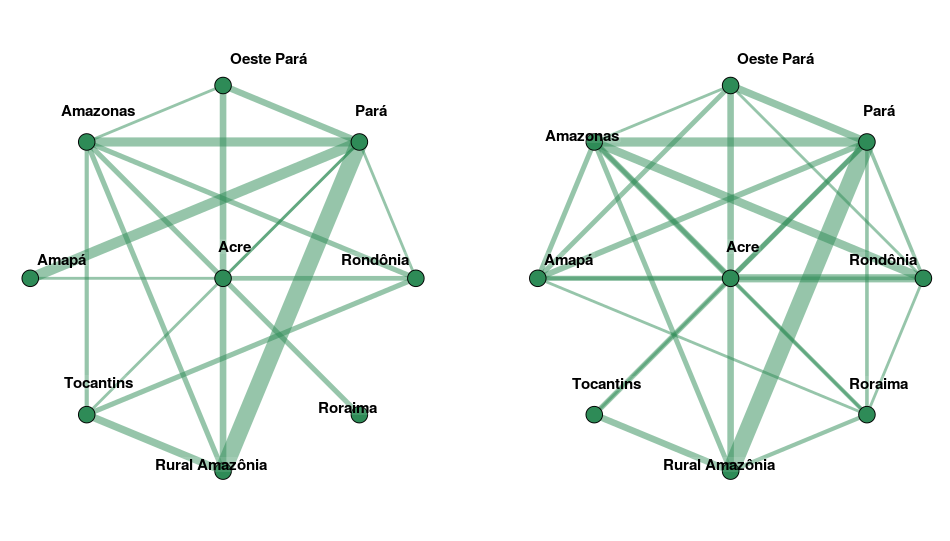
\includegraphics[scale=0.6]{images/norte.png}
\caption{Rede de Coautoria entre as Universidades Federais da \textbf{Região Norte} [P1 e P2]}
\label{rede-norte}
\end{figure}

A inspeção visual (análise gráfica) das redes plotadas traz uma notável impressão do aumento de arestas (ligações) existentes nas coautorias entre as instituições da Região Norte, que pode ser ratificado pelo aumento do número arestas entre P1 e P2, sendo de 17 para 26. É notável a forte relação existente entre a Universidade Federal do Pará e a Univerisdade Federal Rural da Amazônia, em virtude da espessura da arestas, significando uma maior proporção de coautorias existentes dentro da rede em análise. O grau médio da rede variou entre os períodos, considerando sua aferição de 5,77 no P2, apresenta que houve maior conectividade entre os vértices.

%%% VLR (continuar análises)


\begin{table}[H]
\centering
\begin{tabular}{lll}
\hline
\rowcolor[HTML]{C0C0C0} 
\textbf{Métricas} & \textbf{P1} & \textbf{P2} \\ \hline
Qtde. de Vértices & 9           & 9           \\ \hline
Qtde. de Arestas  & 17          & 26          \\ \hline
Grau Médio        & 3.77778     & 5.77778     \\ \hline
Diâmetro          & 9           & 7           \\ \hline
Distância Média   & 1.58333     & 1.27778     \\ \hline
\end{tabular}
\caption{Métricas das redes da Região Norte para P1 e P2}
\end{table}

\section{Região Nordeste}

\begin{figure}[H]
\centering
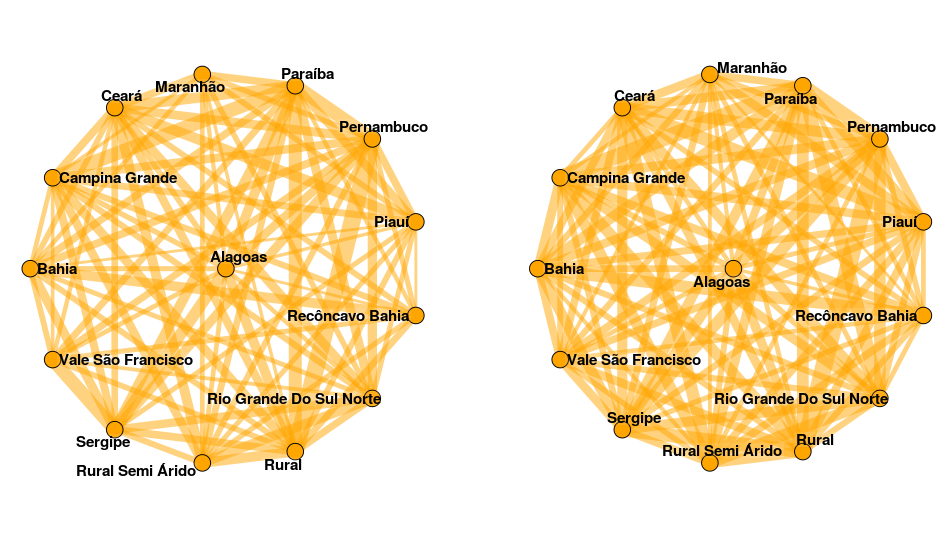
\includegraphics[scale=0.6]{images/nordeste.png}
\caption{Rede de Coautoria entre as Universidades Federais da Região Nordeste [P1 e P2]}
\label{rede-nordeste}
\end{figure}

%(análise e comentários)


\begin{table}[H]
\centering
\begin{tabular}{lll}
\hline
\rowcolor[HTML]{C0C0C0} 
\textbf{Métricas} & \textbf{P1} & \textbf{P2} \\ \hline
Qtde. de Vértices & 14           & 14           \\ \hline
Qtde. de Arestas  & 83           & 91          \\ \hline
Grau Médio        & 11.85714     & 13     \\ \hline
Diâmetro          & 39           & 37           \\ \hline
Distância Média   & 1.08791      & 1     \\ \hline
\end{tabular}
\caption{Métricas das redes da Região Nordeste para P1 e P2}
\end{table}


\section{Região Cento-Oeste}


\begin{figure}[H]
\centering
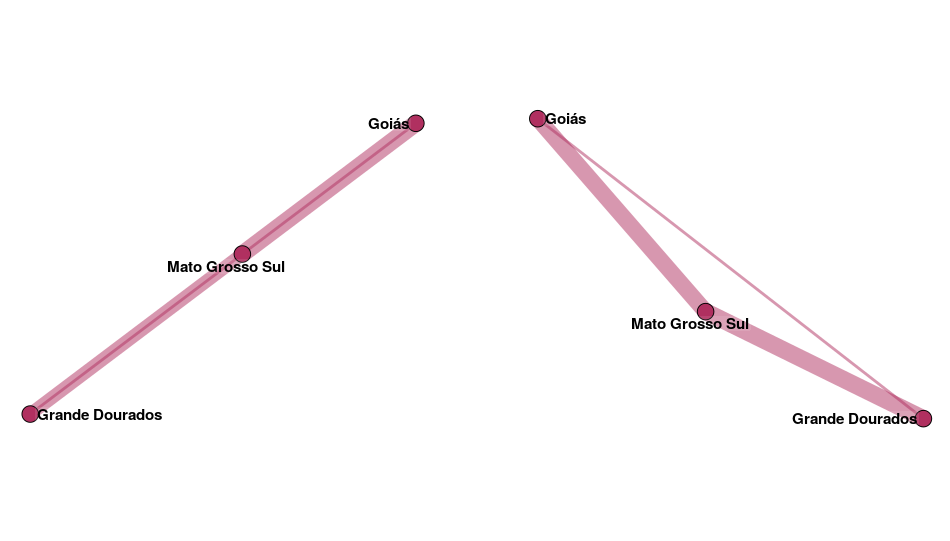
\includegraphics[scale=0.6]{images/centro_oeste.png}
\caption{Rede de Coautoria entre as Universidades Federais da Região Centro-Oeste [P1 e P2]}
\label{rede-centro}
\end{figure}

%(análise e comentários)

\begin{table}[H]
\centering
\begin{tabular}{lll}
\hline
\rowcolor[HTML]{C0C0C0} 
\textbf{Métricas} & \textbf{P1} & \textbf{P2} \\ \hline
Qtde. de Vértices & 3           & 3           \\ \hline
Qtde. de Arestas  & 3           & 3          \\ \hline
Grau Médio        & 2           & 2          \\ \hline
Diâmetro          & 93          & 254         \\ \hline
Distância Média   & 1           & 1            \\ \hline
\end{tabular}
\caption{Métricas das redes da Região Centro-Oeste para P1 e P2}
\end{table}

\section{Região Sudeste}

\begin{figure}[H]
\centering
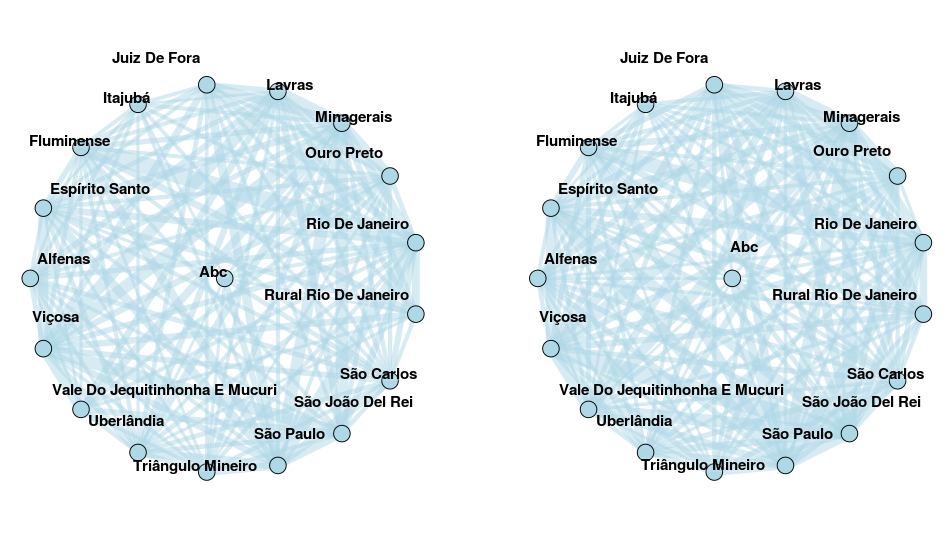
\includegraphics[scale=0.6]{images/sudeste.png}
\caption{Rede de Coautoria entre as Universidades Federais da Região Sudeste [P1 e P2]}
\label{rede-sudeste}
\end{figure}

%(análise e comentários)

\begin{table}[H]
\centering
\begin{tabular}{lll}
\hline
\rowcolor[HTML]{C0C0C0} 
\textbf{Métricas} & \textbf{P1} & \textbf{P2} \\ \hline
Qtde. de Vértices & 18          & 18           \\ \hline
Qtde. de Arestas  & 132         & 142          \\ \hline
Grau Médio        & 14.66667    & 15.77778     \\ \hline
Diâmetro          & 17          & 26           \\ \hline
Distância Média   & 1.13725     & 1.0719     \\ \hline
\end{tabular}
\caption{Métricas das redes da Região Sudeste para P1 e P2}
\end{table}


\section{Região Sul}

\begin{figure}[H]
\centering
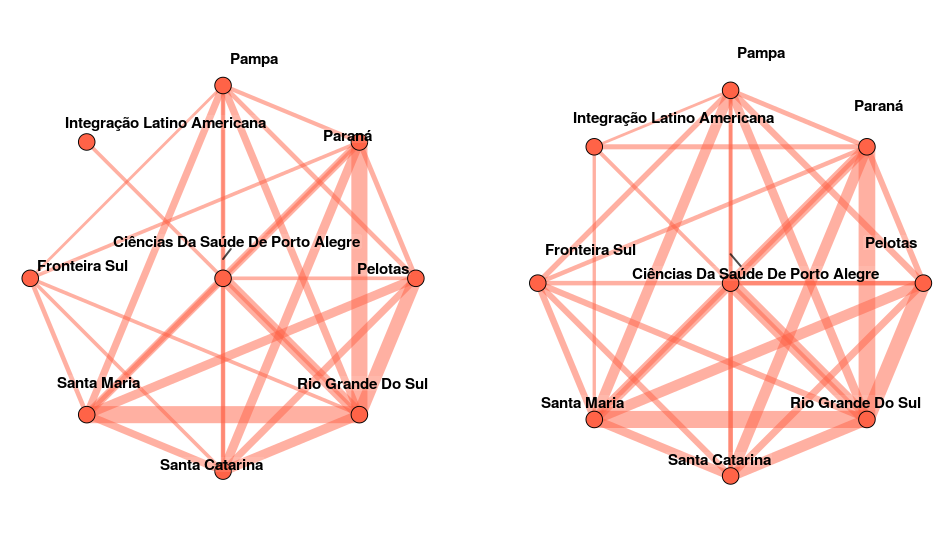
\includegraphics[scale=0.6]{images/sul.png}
\caption{Rede de Coautoria entre as Universidades Federais da Região Sul [P1 e P2]}
\label{rede-sul}
\end{figure}

%(análise e comentários)

\begin{table}[H]
\centering
\begin{tabular}{lll}
\hline
\rowcolor[HTML]{C0C0C0} 
\textbf{Métricas} & \textbf{P1} & \textbf{P2} \\ \hline
Qtde. de Vértices & 9           & 9           \\ \hline
Qtde. de Arestas  & 27          & 31          \\ \hline
Grau Médio        & 6           & 6.88889     \\ \hline
Diâmetro          & 58          & 89           \\ \hline
Distância Média   & 1.25        & 1.13889     \\ \hline
\end{tabular}
\caption{Métricas das redes da Região Sul para P1 e P2}
\end{table}

%%% VLR inserir no apêndice tabela com as Univ. Federais

%\begin{table}[H]
%\begin{tabular}{ll}
%\hline
%\textbf{Universidade Federal}                             & %\textbf{Região} \\ \hline
%Universidade Federal de Goiás                             & Centro-Oeste    \\ \hline
%Universidade Federal de Mato Grosso do Sul                & Centro-Oeste    \\ \hline
%Universidade Federal de Mato Grosso                       & Centro-Oeste    \\ \hline
%Universidade Federal da Grande dourados                   & Centro-Oeste    \\ \hline
%Universidade Federal do Mato Grosso                       & Centro-Oeste    \\ \hline
%Universidade Federal do Mato Grosso do Sul                & Centro-Oeste    \\ \hline
%Universidade Federal do Ceará                             & Nordeste        \\ \hline
%Universidade Federal do Pampa                             & Nordeste        \\ \hline
%Universidade Federal do Piauí                             & Nordeste        \\ \hline
%Universidade Federal de Campina Grande                    & Nordeste        \\ \hline
%Universidade Federal de Alagoas                           & Nordeste        \\ \hline
%Universidade Federal da Bahia                             & Nordeste        \\ \hline
%Universidade Federal do Rio Grande do Norte               & Nordeste        \\ \hline
%Universidade Federal de Sergipe                           & Nordeste        \\ \hline
%Universidade Federal de Pernambuco                        & Nordeste        \\ \hline
%Universidade Federal da Paraíba                           & Nordeste        \\ \hline
%Universidade Federal Rural de Pernambuco                  & Nordeste        \\ \hline
%Universidade Federal Rural do Semi-Árido                  & Nordeste        \\ \hline
%Universidade Federal do Recôncavo da Bahia                & Nordeste        \\ \hline
%Universidade Federal do Maranhão                          & Nordeste        \\ \hline
%Universidade Federal do Vale do São Francisco             & Nordeste        \\ \hline
%Universidade Federal do Pará                              & Norte           \\ \hline
%Universidade Federal do Tocantins                         & Norte           \\ \hline
%Universidade Federal do Acre                              & Norte           \\ \hline
%Universidade Federal do Amazonas                          & Norte           \\ \hline
%Universidade Federal de Rondônia                          & Norte           \\ \hline
%Universidade Federal de Roraima                           & Norte           \\ \hline
%Universidade Federal do Amapá                             & Norte           \\ \hline
%Universidade Federal Rural da Amazônia                    & Norte           \\ \hline
%Universidade Federal do Oeste do Pará                     & Norte           \\ \hline
%Universidade Federal do Espírito Santo                    & Sudeste         \\ \hline
%Universidade Federal de Lavras                            & Sudeste         \\ \hline
%Universidade Federal de Viçosa                            & Sudeste         \\ \hline
%Universidade Federal Fluminense                           & Sudeste         \\ \hline
%Universidade Federal de Uberlândia                        & Sudeste         \\ \hline
%Universidade Federal do Rio de Janeiro                    & Sudeste         \\ \hline
%Universidade Federal de São Carlos                        & Sudeste         \\ \hline
%Universidade Federal de Juiz de Fora                      & Sudeste         \\ \hline
%Universidade Federal de São Paulo                         & Sudeste         \\ \hline
%Universidade Federal Rural do Rio de Janeiro              & Sudeste         \\ \hline
%Universidade Federal de Alfenas                           & Sudeste         \\ \hline
%Universidade Federal de Ouro Preto                        & Sudeste         \\ \hline
%Universidade Federal do Estado do Rio de Janeiro          & Sudeste         \\ \hline
%Universidade Federal do Abc                               & Sudeste         \\ \hline
%Universidade Federal do Triângulo Mineiro                 & Sudeste         \\ \hline
%Universidade Federal dos Vales do Jequitinhonha E Mucuri  & Sudeste         \\ \hline
%Universidade Federal de Itajubá                           & Sudeste         \\ \hline
%Universidade Federal de São João Del-Rei                  & Sudeste         \\ \hline
%Universidade Federal de S. Carlos                         & Sudeste         \\ \hline
%Universidade Federal de Minas Gerais                      & Sudeteste       \\ \hline
%Universidade Federal de Santa Maria                       & Sul             \\ \hline
%Universidade Federal de Santa Catarina                    & Sul             \\ \hline
%Universidade Federal do Rio Grande do Sul                 & Sul             \\ \hline
%Universidade Federal de Pelotas                           & Sul             \\ \hline
%Universidade Federal do Rio Grande                        & Sul             \\ \hline
%Universidade Federal do Paraná                            & Sul             \\ \hline
%Universidade Federal de Ciências da Saúde de Porto Alegre & Sul             \\ \hline
%Universidade Federal da Fronteira Sul                     & Sul             \\ \hline
%Universidade Federal da Integração Latino-Americana       & Sul             \\ \hline
%\end{tabular}
%\end{table}

\bibliographystyle{agsm}
\bibliography{references}

\end{document}
